\documentclass[11pt]{article}

\usepackage{graphicx}

\usepackage[backend=biber,style=ieee]{biblatex}
\addbibresource{refs.bib}

\usepackage{comment}
\usepackage{pdflscape}

\begin{document}

\title{{\Huge Updated Project Plan}\\ Verification of Digital Designs}
\author{Tjark Petersen}
\date{\today}

\maketitle


\begin{comment}
- verification important -> not only for functional correctness, but required for safety-critical systems
- in the critical path of the development process \cite{bergeron2012writing}
- consumes more than 2/3 of the development time \cite{bergeron2012writing}
- dedicated verification engineers
- intricate process, not any more just writing a testbench with some directed test cases
- complex environments, complex SoCs, random stimulus, coverage-driven verification, formal verification, etc.
- abstraction can help to manage complexity \cite{bergeron2012writing}
- but we have balance control and abstraction \cite{bergeron2012writing}



- HVLs were introduced to abstract and ease testbench development
- intially co-simulation based like Vera added crv, OOP, etc.
- today SV merged SuperLog and Vera -> single language

- SV alone provides primitives for creation of best practice test environments
- but no guidlines of how to do so -> no reuse
- UVM introduces framework for creation of sophisticated testbenches in SV which encourage reuse by providing guidelines and class hierarchies \cite{flake2020a}
- standard from 2017




- "all verification projects present a recurring set of challenges; hence, valuable time and effort are saved by reusing code common to all environments. This is achieved with a software library that provides verification facilities such as error reporting and communications handshaking" \cite{flake2020a}


\end{comment}

Functional verification is an integral part of the development process of a digital system. It is not only needed to ensure functional correctness but also required to prove the fulfillment of specific safety requirements in safety-critical systems. 
With ever more complex heterogeneous systems-on-chips (SoCs) coming with a large set of functional requirements, the task of verification has gotten a bottleneck in the development process requiring up to 2/3 of the development time \cite{bergeron2012writing}.

Simulation based verification techniques have evolved from simple directed testbenches to more sophisticated approaches using constrained random stimulus alongside monitoring of functional coverage, based on the stimulus as well as assertions. 
The \textit{Universal Verification Methodology} (UVM) is a widely adopted IEEE standard which provides a framework for creating sophisticated testbenches in SystemVerilog that encourages reuse by providing guidelines and templates for common building blocks \cite{flake2020a}. 

While work is in progress of enabling the UVM on Verilator, an open-source (System)Verilog simulator, the UVM in SystemVerilog is for now only fully supported by commercial simulators.
In the open-source community, the \textit{cocotb} project provides a Python-based co-simulation environment, while the \textit{pyUVM} project aims to provide a Python-based UVM-like framework. The \textit{pyVSC} project adds random stimulus generation and coverage collection capabilities. Other projects like \textit{Chisel} or \textit{SpinalHDL} have their own testbench frameworks, which only provide barebones means to control a simulation and drive stimulus. The \textit{ChiselVerify} project added some features required for modern verification on top of the \textit{chiseltest} framework like coverage collection and constrained random stimulus generation. With chiseltest getting deprecated, the future of ChiselVerify is uncertain.

Initial talks with two Copenhagen based companies working with verification have shown that the UVM is not perfect. The guidelines are still quite loose, leading to different ways of achieving the same goal. For instance the implementation of a scoreboard isn't standardized. The Register Abstraction Layer (RAL) wasn't received as being complete either, leading to both companies developing internal extensions.

While Python is a language with a low entry barrier, it does not scale well with complex systems such as large testbench environments where features like compile-time type safety can circumvent run-time crashes and provide larger confidence in the correctness of the implemented code. This is especially important when reuse is encouraged such that the internals of verification components aren't always known to the developer. Instead a statically typed language should be used. On the other hand, the verbosity of the language should be minimal while offering garbage collection and a rich standard library to ease the development process. 

This opens the opportunity to reconsider the abstractions behind the UVM as well as their respective implementation in the context of a new open-source framework. This framework should accept synthesizable SystemVerilog designs to make it as accessible as possible, given that (System)Verilog is the most widely used language for digital design and used as an intermediate language by other hardware description languages like Chisel, MyHDL or SpinalHDL.

\textit{Scala} is a language that fits the requirements for a compiled, garbage-collected language with a strong type system. At its core, the language is simple and concise but it offers more advanced features like functional programming. The language is furthermore especially friendly to DSLs, which should allow for natural APIs for the user of a verification framework. It it therefore chosen as the language for the implementation of the proposed framework.


\noindent The framework shall provide the following features:

\begin{itemize}
    \item \textbf{Backend}: a backend to interface with \textit{Verilator} simulations
    \item \textbf{Concurrency}: support for concurrency in the testbench
    \item \textbf{Phasing}: support for different simulation phases
    \item \textbf{Components}: building blocks for common verification components like drivers, monitors, sequencers, etc.
    \item \textbf{Utilities}: utilities for tasks like error reporting, communication between threads and easy configuration
\end{itemize}


\noindent A timeline for the execution of the project is provided on the next page in Figure \ref{fig:gantt} in the form of a Gantt chart.

\begin{landscape}
    \pagestyle{empty}%
    \begin{figure}
        \hspace{-2.5cm}
        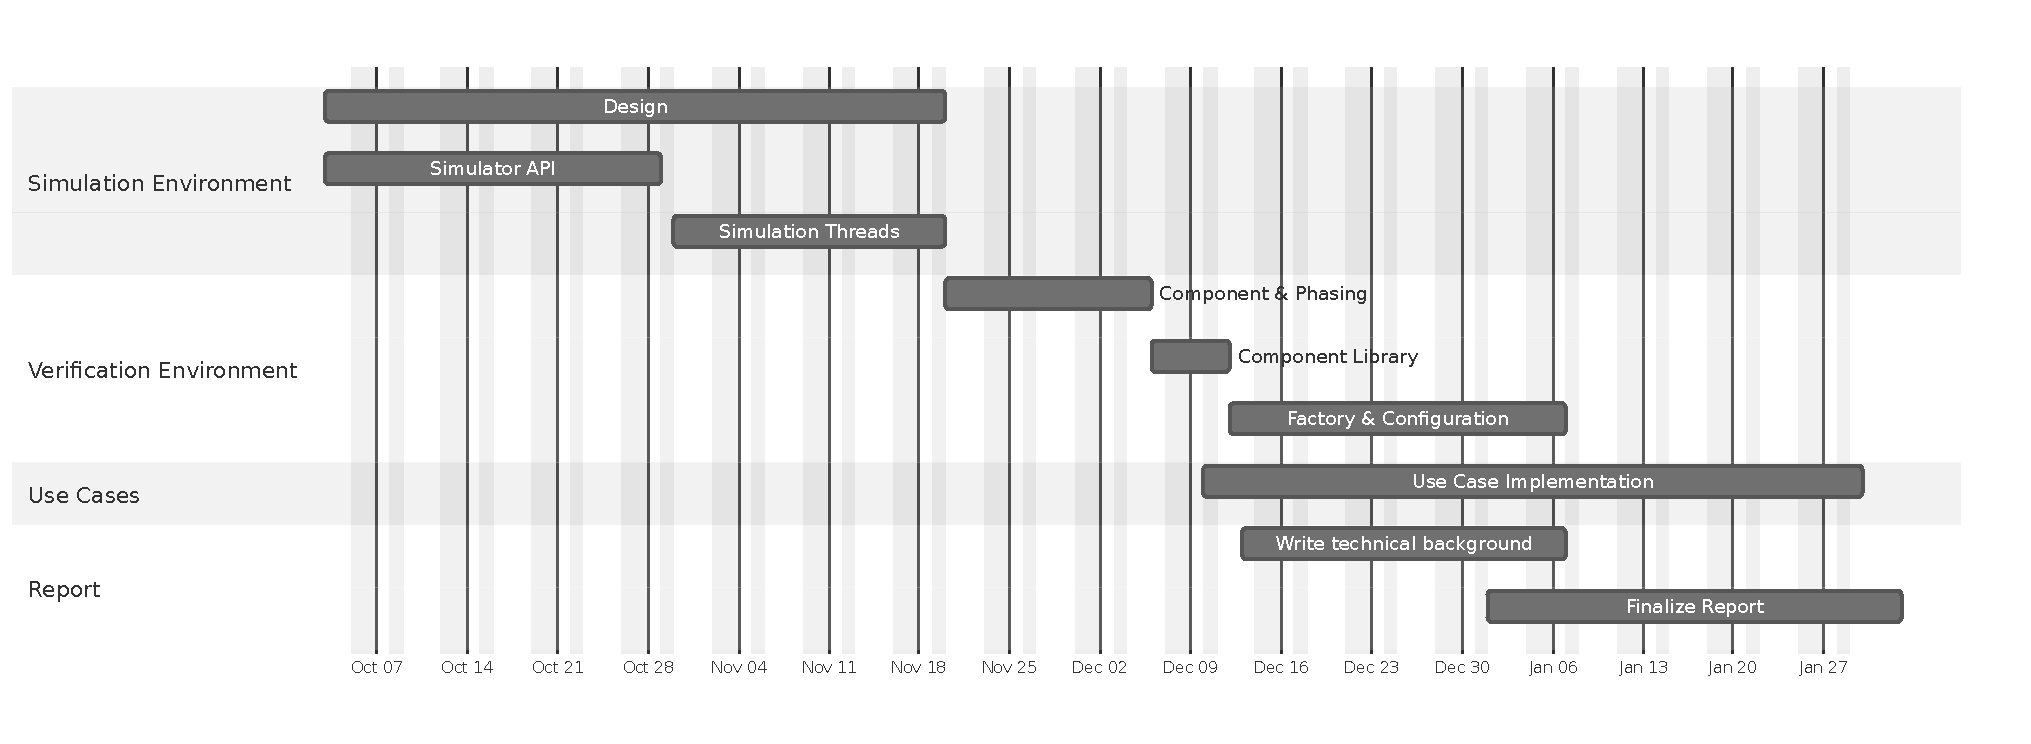
\includegraphics[width=24cm]{gantt.pdf}
        \caption{Gantt chart for the project execution.}
        \label{fig:gantt}
\end{figure}
\end{landscape}


\printbibliography

\end{document}